\documentclass[german]{latex4ei/latex4ei_sheet}
\usepackage{stix}
\usepackage[ngerman]{babel} 
% set document information
\title{Hochfrequenztechnik \\ Cheat Sheet}
\author{Raoul Duke}
\myemail{0x4723@gmail.com}
\mywebsite{www.github.com/doppelplus/CheatSheets}

\begin{document}

\maketitle
\section{Allgemeines}
    \begin{sectionbox}{\textbf{Frequenz und Wellenlänge}}
        \item Lichtgeschwindigkeit: $c = 299\,792\,458\,m/s$
        \item $F = \frac{c}{\lambda} \rightarrow \lambda = \frac{c}{F}$
    \end{sectionbox}
    \begin{sectionbox}{\textbf{dBm}}
        \item dBm (Dezibel Milliwatt) ist die Einheit des Leistungspegels LP, der das Verhältnis einer Leistung P im Vergleich zur Bezugsleistung von 1\,mW beschreibt. 
        \item $L_p[dBm] = 10\lg\left(\frac{P}{1\,mW}\right)$
        \item $P[mW] = 10^{\left(\frac{L_p[dBm]}{10}\right)}\cdot 1\,mW$
        \item \begin{symbolbox} {Rechnen mit dBm oder dBW}
            \item $dB \pm dB = dB$
            \item $dBm \pm dB = dBm$
            \item $dBm - dBm = dB$
            \item $dBm + dBm : nicht\, definiert$
        \end{symbolbox}
    \end{sectionbox}

\section{(Wideband) Code Division Multiple Access}
    \begin{sectionbox}
        \begin{bluebox}{Signalspreizung}
            \item Direct Sequence CDMA.
            \item Datenstrom wird bei Sender \& Empfänger mit Spreizcode multipliziert.
            \item Mehrere Datenströme können im gleichen Frequenzband übertragen werden.
            \item 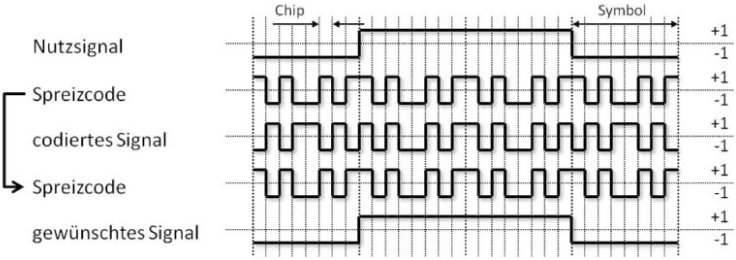
\includegraphics[width=185px]{img/Signalspreizung.png}
            \item Das Spektrum des gespreizten Nutzsignals ist um ein vielfaches breiter, als das originäre Signal. 
        \end{bluebox}
        \begin{symbolbox}{Formelzeichen}
            \item Spreizfaktor: $SF$
            \item Processing Gain: $PG$
            \item Chiprate: $b_c$
            \item Nutzdatenrate: $b_n$
            \item Störabstand: $SIR$
            \item Signalleistung: $S$
            \item Anzahl der aktiven Signale in der Funkzelle: $N$
            \item Mittlere Nutzenergie pro Bit: $E_b$
            \item Rauschenergie pro Bit: $N_0$
        \end{symbolbox}
        
        \begin{bluebox}
            \item $PG = 10\log SF\,dB$
            \item $SF = \frac{b_c}{b_n}$
            \item $SIR = \frac{S}{(N-1)\cdot S}= \frac{1}{1 N-1}$
            \item $\frac{E_b}{N_0} = \frac{S/b_N}{((N-1)S)/b_c} = \frac{1}{N-1}\cdot \frac{b_c}{b_N} = SIR \cdot SF$
            \item $10 \cdot \log \left(\frac{E_b}{N_0}\right) = 10\cdot \log (SIR)+ PG\,dB$
            \item $N = \frac{b_C}{E_b/N_0\cdot b_N}+1$
        \end{bluebox}
    \end{sectionbox}
\vspace{4cm}
    \section{Orthogonal Frequency Division Multiplexing}
    \begin{sectionbox}
        \begin{symbolbox}{Formelzeichen}
            \item Bandbreite: $W$
            \item Anzahl der Unterträger: $n$
            \item Breite der Unterträger: $B_U$+
            \item Symboldauer: $T_D$
            \item Zeitintervall: $T_S$ 
            \item Datensymbole: $D_0 \dots D_{-1}$
            \item Grundfrequenz: $f_G$
            \item Kanalfrequenz: $f_k$
            \item Abtastrate: $f_A$
        \end{symbolbox}
        
        \begin{bluebox}{Formeln}
            \item $B_U = \frac{W}{n}$
            \item $f_k =k \cdot f_G$\quad $k$ ganzzahlig mit $-\frac{n}{2}\geq k \geq \frac{n}{2}-1$ 
            \item $f_A = f_G = \frac{1}{T_S}$
            \item $T_S = n \cdot T_D$
            \item $\Delta f = f_k - f_{k-1} = k\cdot f_G -(k-1)\cdot f_G = f_G$
        \end{bluebox}
    \end{sectionbox}

    \section{Funkfelddämpfung}
    \subsection{Allgemeines}
    \begin{sectionbox}
        \begin{symbolbox}{Formelzeichen}
            \item 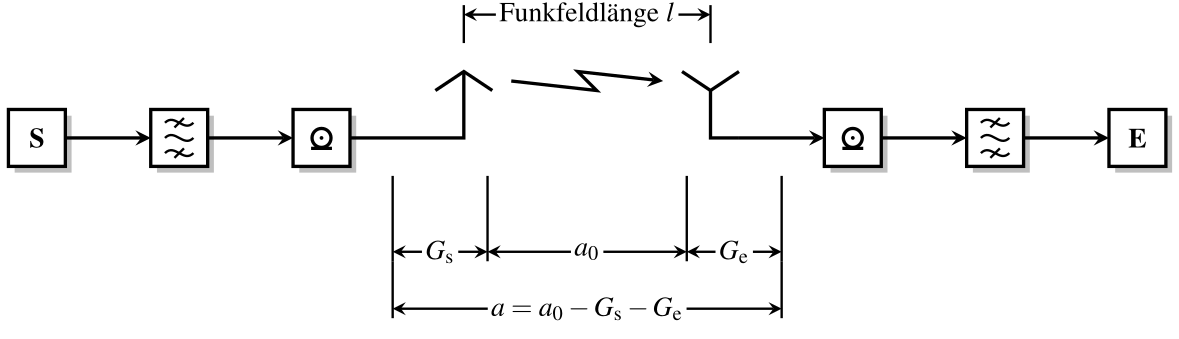
\includegraphics[width=185px]{img/Funkuebertragungssystem.png}
            \item Gewinn der Sendeantenne: $G_s$
            \item Gewinn der Empfangsantenne: $G_e$
            \item Sendeleistung: $P_s$
            \item Empfangsleistung: $P_e$
            \item Funkfelddämpfung: $a$
            \item Freiraumdämpfung: $a_0$
        \end{symbolbox}
        
        \begin{bluebox}{Formeln}
            \item $a = \frac{P_s}{P_e} = \frac{(4\pi l)^2}{\lambda^2 G_e G_s}$ \textbf{als Faktor}.
            \item $a = P_s - P_e = 20\lg \frac{4\pi l}{\lambda}-G_s-G_e$ \textbf{in dB}.
            \item $a_0 = 20\lg \frac{4\pi l}{\lambda} = 20\lg \frac{4\pi\cdot l \cdot f}{c}$
        \end{bluebox}
    \end{sectionbox}
    \begin{sectionbox}   
        \subsection{Einwegausbreitung}
    \begin{symbolbox}{Einwegeausbreitung}
        \item Übertragungsfunktion (Einwegausbreitung):\\ $H(f) = a_1 e^{j\varphi_1} = a_1 e^{-j 2 \pi f \tau_1}$
        \item Laufzeit: $\tau_1$
        \item Komplexe Amplitude der Übertragungsfunktion: $a_1 = \frac{4\pi d_1}{\lambda}\cdot \frac{1}{\sqrt{G_s G_e}}$
        \item Phasenwinkel der Übertragungsfunktion: $\varphi_1$
        \item $|H(f)| = a_1$
        \item Laufweg: $d_1\tau_1 \cdot c$
    \end{symbolbox}
\end{sectionbox}
    
\begin{sectionbox}{\subsection{Zweiwegeausbreitung}}
        \item 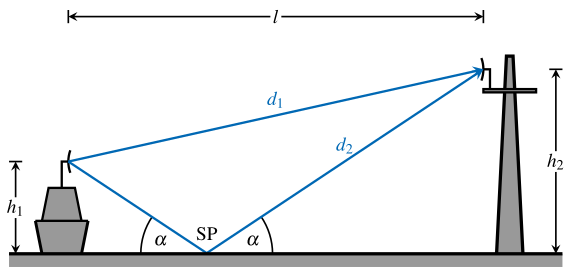
\includegraphics[width=185px]{img/Zweiwegeausbreitung.png}
        \item Impulsantwort: $h(t) = a_1 \delta(t-\tau_1)+ a_2 \delta(t-\tau_2)$
        \item Phasendifferenz: $\Delta \varphi = 2 n \pi$ mit $n \in \mathbb{N} \rightarrow$ Feldstärke verdoppelt.
        \item Phasendifferenz: $\Delta \varphi = (2n+1) \pi$ mit $n \in \mathbb{N} \rightarrow$ Feldstärke ausgelöscht.
\end{sectionbox}
\section{Verfügbarkeit und Zuverlässigkeit}
    \begin{sectionbox}{\subsection{Verfügbarkeit}}
        \item 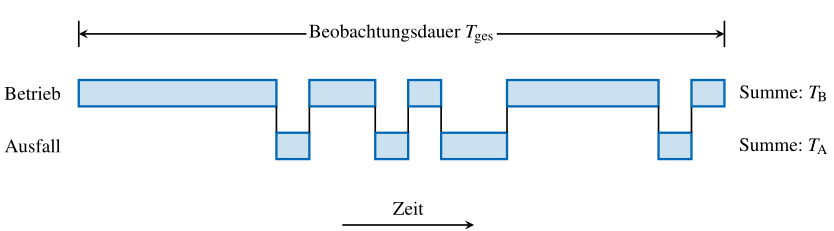
\includegraphics[width=185px]{img/Verfuegbarkeit.png}
        \item Verfügbarkeit: $V= \frac{T_B}{T_{ges}} = \frac{T_B}{T_b+T_A} = 1-\frac{T_A}{T_{ges}}$
        \item Verfügbarkeit Serienschaltung: $V_{ges} = \prod\limits_{i=1}^N V_i $
        \item Verfügbarkeit Paralellschaltung: $V_{ges} = 1-\prod\limits_{i=1}^N (1-V_i) $
    \end{sectionbox}
    \begin{sectionbox}{\subsection{Zuverlässigkeit}}
        \item \begin{quote}
            Die Zuverlässigkeit ist die Wahrscheinlichkeit, dass ein System innerhalb eines
            gegebenen Zeitabschnitts keinen Ausfall aufweist. Eine Messgröße für die 
            Zuverlässigkeit ist der mittlere Abstand zwischen zwei Ausfällen, die Mean Time Between Failures (MTBF).
            Zusammen mit der mittleren Instandsetzungsdauer (Mean Time To Repair) ergibt sich:
        \end{quote}
        $V = \frac{MTBF}{MTBF+MTTR}$
    \end{sectionbox}
\section{Richtfunksysteme}
    \begin{sectionbox}
        \item 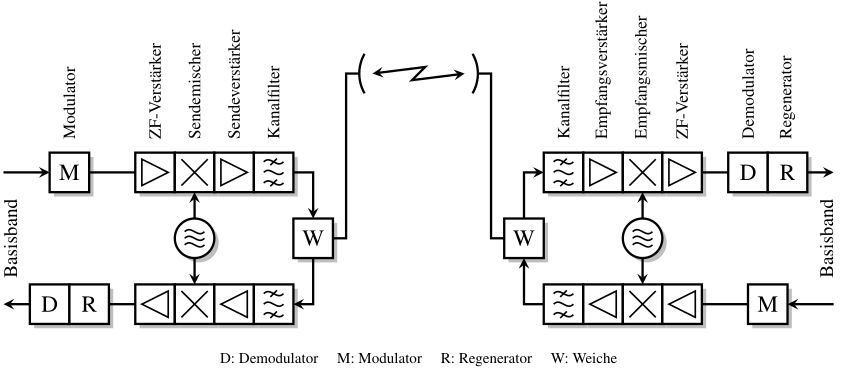
\includegraphics[width=185px]{img/Richtfunk.png}
    \end{sectionbox}
\section{Satellitenfunk}
    \begin{sectionbox}{\subsection{Satellitenbahnen}}
       \item 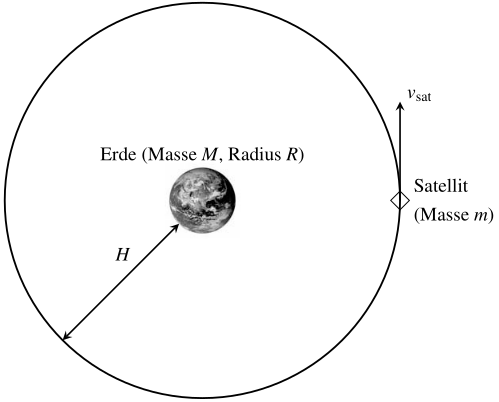
\includegraphics[width=180px]{img/Satellitenumlauf.png}
       \item Gravitationskonstante: $\gamma_s = 6,67\cdot 10^{-11}\, Nm^2/kg^2$
       \item Umlaufzeit: $T = 2\pi \sqrt{\frac{(R+H)^3}{\gamma_s M_E}}$
       \item Bahngeschwindigkeit: $v_{sat} = 2\pi \frac{H+R}{T}$
       \item Umlaufzeit Erde: $T \approx 1,4\,h \left( 1+\frac{H}{6378\,km}\right)^{\frac{3}{2}}$
       \item $H = \sqrt[3]{\frac{T^2}{4\pi^2}\gamma_s M_E - R}$
    \end{sectionbox}
    \begin{sectionbox}{EIRP}
        \item Alles in dB!
        \item Boltzmann-Konstante: $k_B = 228,6\,dB(1K/Ws)$
        \item Güte: $(G_E-T_E)$ 
        \item Margin: $M$
        \item Zusatzdämpfung: $a_z$
        \item Rauschbandbreite: $B_r = 10 \lg(Bandbreite)$
        \item Rauschleistung: $N = kB_rT_e$
        \item Trägerleistung: $C = P_s G_s G_e/a_0 a_z$
        \item Störabstand dez: $C/N = \frac{P_s G_s G_e}{k_B T_e a_0 a_z M}$
        \item Störabstand log: $C/N = EIRP + (G_e-T_e)-a_0-a_z-M-B_r+k_B$
        \item Gewinn: $G = EIRP - P$
        \item Bei $\lim\limits_{C/N\rightarrow 0}$ : $EIRP = -(G_E-T_E) + a_0 + B_r + M + a_z - k_B$    
    \end{sectionbox}
\section{Mikrowellentechnik}
    \begin{sectionbox}{Ebene Wellen im Leiter}
        \item Permeabilität: $\mu$
        \item Permeabilität für Vakuum: $\mu_o$
        \item Leitwert für Kupfer: $\kappa_{Cu} = 5,8 \cdot 10^7\, S/m$
        \item Leitwert für Aluminium: $\kappa_{Al} = 3,66 \cdot 10^7\, S/m$
        \item Eindringtiefe: $\delta = \sqrt{\frac{2}{\omega \kappa \mu}}$
        \item Eindringtiefe für Kupfer: $\delta_{Cu} = \frac{66,085\,\mu m}{\sqrt{\frac{f}{MHz}}}$
        \item Eindringtiefe für Aluminium: $\delta_{Al} = \frac{83,249\,\mu m}{\sqrt{\frac{f}{MHz}}}$
        \item Oberflächenwiderstand: $R_0 = \frac{1}{\kappa \cdot \delta} = \sqrt{\frac{\omega\cdot \mu}{2\cdot \kappa}}$
    \end{sectionbox}
    \begin{sectionbox}{Geführte Wellen}
        \item Bandleitungshöhe: h
        \item Relative Permeabilität eines Substrats: $\varepsilon_r$
        \item Feldwellenwiderstand: $Z_F = Z_0 \cdot \sqrt{\frac{\mu_r}{\epsilon_r}}$
    \end{sectionbox}

\end{document}